\section{Relative Hazard and Survival Frontiers}
\subsection{Global Persistence Is Independent of Allocation}
We begin with the property shared by every balanced companion. No choice of the harmful pair changes the number of surviving descendants: random, adversarial, protective, and mixed parents all leave the same global population. Local extinction must therefore come from placement rather than from exhausting the complete-period supply.
Let $N_k=|\mathcal G_k|$ and assume $N_0>0$. Installing $r_k$ gives
\begin{equation*}
\begin{aligned}
N_{k+1}
&=\sum_{g\in\mathcal G_k}(r_k-2)
&&[\text{Exactly Two Copies Removed Per Parent}]\\
&=(r_k-2)N_k.
&&[\text{Simplification}]
\end{aligned}
\end{equation*}
Consequently,
\begin{equation*}
\begin{aligned}
N_k
&=N_0\prod_{i < k}(r_i-2)
&&[\text{Iteration}]\\
& > 0
&&[N_0>0;\ r_i\ge5]\\
&\longrightarrow\infty.
&&[\text{Every Factor Is At Least }3]
\end{aligned}
\end{equation*}
Thus
\begin{equation*}
\text{global 2-gap persistence holds for every adversarial schedule.}
\qquad[\text{Q.E.D.}]
\end{equation*}
The complete proof record appears in Appendix~A.1. The corresponding real-sieve count is proved in \href{https://github.com/thiagomata/prime-numbers/blob/master/articles/chapter6/gap-dynamics.md#52-exact-non-recursive-global-count}{Gap Dynamics \S{}5.2} \cite{gapdynamics2026}.
\subsection{Local Destruction Relative to Random}
Two quantities must be distinguished. If $L_r > 0$ gaps are present in a specified finite population and $H_r$ are destroyed, its observed fraction is
\begin{equation*}
\widehat f_r:=\frac{H_r}{L_r},
\qquad \widehat w_r:=\frac{r\widehat f_r}{2}.
\end{equation*}
The probability model instead uses the conditional lineage hazard $f_r$ defined in Section~2.1. Balanced random selection has conditional destruction rate
\begin{equation*}
d_r:=\frac2r.
\end{equation*}
The dimensionless worse-than-random factor is
\begin{equation*}
w_r
:=\frac{f_r}{d_r}
=\frac{rf_r}{2}.
\end{equation*}
This is the meaningful adversariality scale because the benchmark itself shrinks as filters grow:
\begin{equation*}
\begin{aligned}
w_r=0
&\Longleftrightarrow f_r=0
&&[\text{Protective Endpoint}],\\
w_r=1
&\Longleftrightarrow f_r=2/r
&&[\text{Random Benchmark}],\\
w_r=r/2
&\Longleftrightarrow f_r=1
&&[\text{Complete Local Destruction}].
\end{aligned}
\end{equation*}
The range $0\le w_r\le r/2$ compares conditional damage with the neutral law. The analogous observed score $\widehat w_r$ can fluctuate above one even for a random filter. An observed fraction does not by itself establish the conditional probability of destruction of a particular child.
\subsubsection*{Absolute Adversarial/Random Share as a Specialization}
Fix a target: either a square-safe window or one distinguished head position. At filter $r$, let
\begin{equation*}
0\le \alpha_r\le 1
\end{equation*}
be the adversarial share. The remaining share $1-\alpha_r$ uses the balanced random choice.
This can be interpreted parent by parent or as a marginal mixture for one locally relevant lineage. For the cumulative product studied below, mixture choices for a tracked lineage are independent from one filter to the next. The one-lineage calculation at each filter is then the same:
- under adversarial selection, its target child is destroyed; - under balanced random selection, that child survives with probability $1-2/r$.
The model therefore assumes that the adversarial branch is strong enough to identify and kill the locally relevant child. That is exactly what makes it an adversarial comparison rather than a description of the real filter.
Its total local destruction rate and relative factor are
\begin{equation*}
\begin{aligned}
f_r
&=\alpha_r+(1-\alpha_r)\frac2r,\\
w_r
&=\frac r2f_r\\
&=1+\frac{r-2}{2}\alpha_r.
\end{aligned}
\end{equation*}
Thus a fixed absolute share $\alpha_r=\alpha > 0$ does not represent a fixed amount worse than random. It makes $w_r$ grow linearly like $\alpha r/2$. This is why the fixed-share model is asymptotically fatal for an essentially trivial reason; the nontrivial question is how rapidly $w_r$ itself may grow.
\subsection{The General Cumulative Local-Hazard Law}
Follow one eligible candidate through successive filters. By the conditional hazard definition, its next survival probability is
\begin{equation*}
s_r=1-f_r=1-\frac{2w_r}{r}.
\end{equation*}
Assume $f_r < 1$ for every filter in the tracked chain. Define the cumulative local hazard
\begin{equation*}
D(Q)
:=\sum_{r < Q}-\log(1-f_r)
=\sum_{r < Q}-\log\left(1-\frac{2w_r}{r}\right).
\end{equation*}
The complete survival factor is exactly
\begin{equation*}
\begin{aligned}
P(Q)
&=\prod_{r < Q}(1-f_r)
&&[\text{Conditional Probability Chain Rule}]\\
&=\exp\left(\sum_{r < Q}\log(1-f_r)\right)
&&[\text{Product To Sum}]\\
&=e^{-D(Q)}.
&&[\text{Definition Of }D(Q)]
\end{aligned}
\qquad[\text{Q.E.D.}]
\end{equation*}
There is also a deterministic version. For a fixed nested cohort with no births or immigration, $L_{r^+}=L_r(1-\widehat f_r)$ telescopes to the ratio of final to initial cohort size. This is an observed ratio, not a marginal probability. Changing the target window or introducing new descendants breaks that telescope unless an additional accounting identity is proved.
The Prime Number Theorem, the prime harmonic estimate, and their partial-summation consequences used here and below are classical; we use Hardy and Wright \cite{hardywright2008}.
For the random benchmark $w_r=1$,
\begin{equation*}
\begin{aligned}
D_{\mathrm{random}}(Q)
&=\sum_{r < Q}-\log\left(1-\frac2r\right)\\
&=2\log\log Q+O(1),
\end{aligned}
\end{equation*}
and therefore
\begin{equation*}
P_{\mathrm{random}}(Q)
\asymp\frac{C}{(\log Q)^2}.
\end{equation*}
The absolute adversarial/random mixture from Section~3.2 is recovered because
\begin{equation*}
1-f_r
=(1-\alpha_r)\left(1-\frac2r\right).
\end{equation*}
If
\begin{equation*}
A(Q):=\sum_{r < Q}-\log(1-\alpha_r),
\end{equation*}
then
\begin{equation*}
\begin{aligned}
D_{\mathrm{adversarial/random}}(Q)
&=D_{\mathrm{random}}(Q)+A(Q),\\
P_{\mathrm{adversarial/random}}(Q)
&\asymp\frac{C}{(\log Q)^2}e^{-A(Q)}.
\end{aligned}
\end{equation*}
Thus the earlier $A(Q)$ is an excess hazard created by one particular policy mixture. The primary quantity is $D(Q)$, which also applies when no policy label $\alpha_r$ exists.
If one filter has $f_r=1$, local extinction is immediate and the cumulative hazard is infinite from that point.
The complete proof record appears in Appendix~A.2.
\subsection{Every Fixed Finite Worsening Factor Survives}
The random destruction rate shrinks like $2/r$. We first ask what happens when the local filter is a fixed number of times worse than that benchmark. With a quadratic supply of eligible starts and blind placement, every fixed factor still leaves occupied square windows. If head candidates remain available and successive layers mix adequately, the head also returns to a 2-gap infinitely often.
Let $w\ge 0$ be fixed and suppose
\begin{equation*}
f_r=\frac{2w}{r}
\end{equation*}
for all sufficiently large filters. A finite prefix is absorbed into a positive constant. Since the quadratic error terms are summable over primes,
\begin{equation*}
\begin{aligned}
D_w(Q)
&=\sum_{r < Q}-\log\left(1-\frac{2w}{r}\right)
&&[\text{Definition Of }D(Q)]\\
&=2w\sum_{r < Q}\frac1r+O(1)
&&[\text{Taylor Expansion; Summable Remainder}]\\
&=2w\log\log Q+O(1).
&&[\text{Prime Harmonic Sum}]
\end{aligned}
\end{equation*}
Therefore
\begin{equation*}
P_w(Q)\asymp\frac{C_w}{(\log Q)^{2w}}.
\end{equation*}
For a square window with $B(Q)\asymp C_0Q^2$ eligible lineages,
\begin{equation*}
\lambda_w(Q)
\asymp
C_0\frac{Q^2}{(\log Q)^{2w}}
\longrightarrow\infty
\end{equation*}
for every finite $w$. The growth is strong enough to make the standard empty-window bound summable, so only finitely many square windows are empty almost surely under the blind-placement premise.
For a distinguished head with baseline availability bounded below,
\begin{equation*}
\Pr(H_Q)\asymp\frac{C_w}{(\log Q)^{2w}}.
\end{equation*}
The sum of this probability over prime heads diverges for every finite $w$. Under adequate mixing, head 2-gaps therefore recur infinitely often almost surely.
Thus
\begin{equation*}
\text{there is no finite constant-factor maximum worse than random.}
\qquad[\text{Q.E.D.}]
\end{equation*}
A filter that is twice, ten times, or one million times worse than the random rate still lies in the same asymptotic survival class once $r$ is sufficiently large. The nontrivial transition begins only when $w_r$ grows with $r$.
The complete proof record appears in Appendix~A.3.
The fixed-factor conclusion is not only asymptotic; it is visible in the square-window occupancy itself. The figure below plots $\log_{10}\lambda_w(Q)$ against $\log_{10}Q$ for the fixed factors $w=1,3,6,10$, a constant $1\%$ adversarial share, and the $c=1$ frontier $w_r=1+\log r$. Every fixed finite $w$ climbs without bound -- $w=6$ and $w=10$ visibly dip first, because $Q^2$ must first outgrow $(\log Q)^{2w}$ -- while the constant share collapses rapidly and the exact $c=1$ boundary declines only logarithmically: $\lambda_1(Q)\asymp C/(\log Q)^2\to0$. This is the failure-side boundary derived in Section~3.5, not a surviving curve.
\begin{figure}[htbp]
\centering
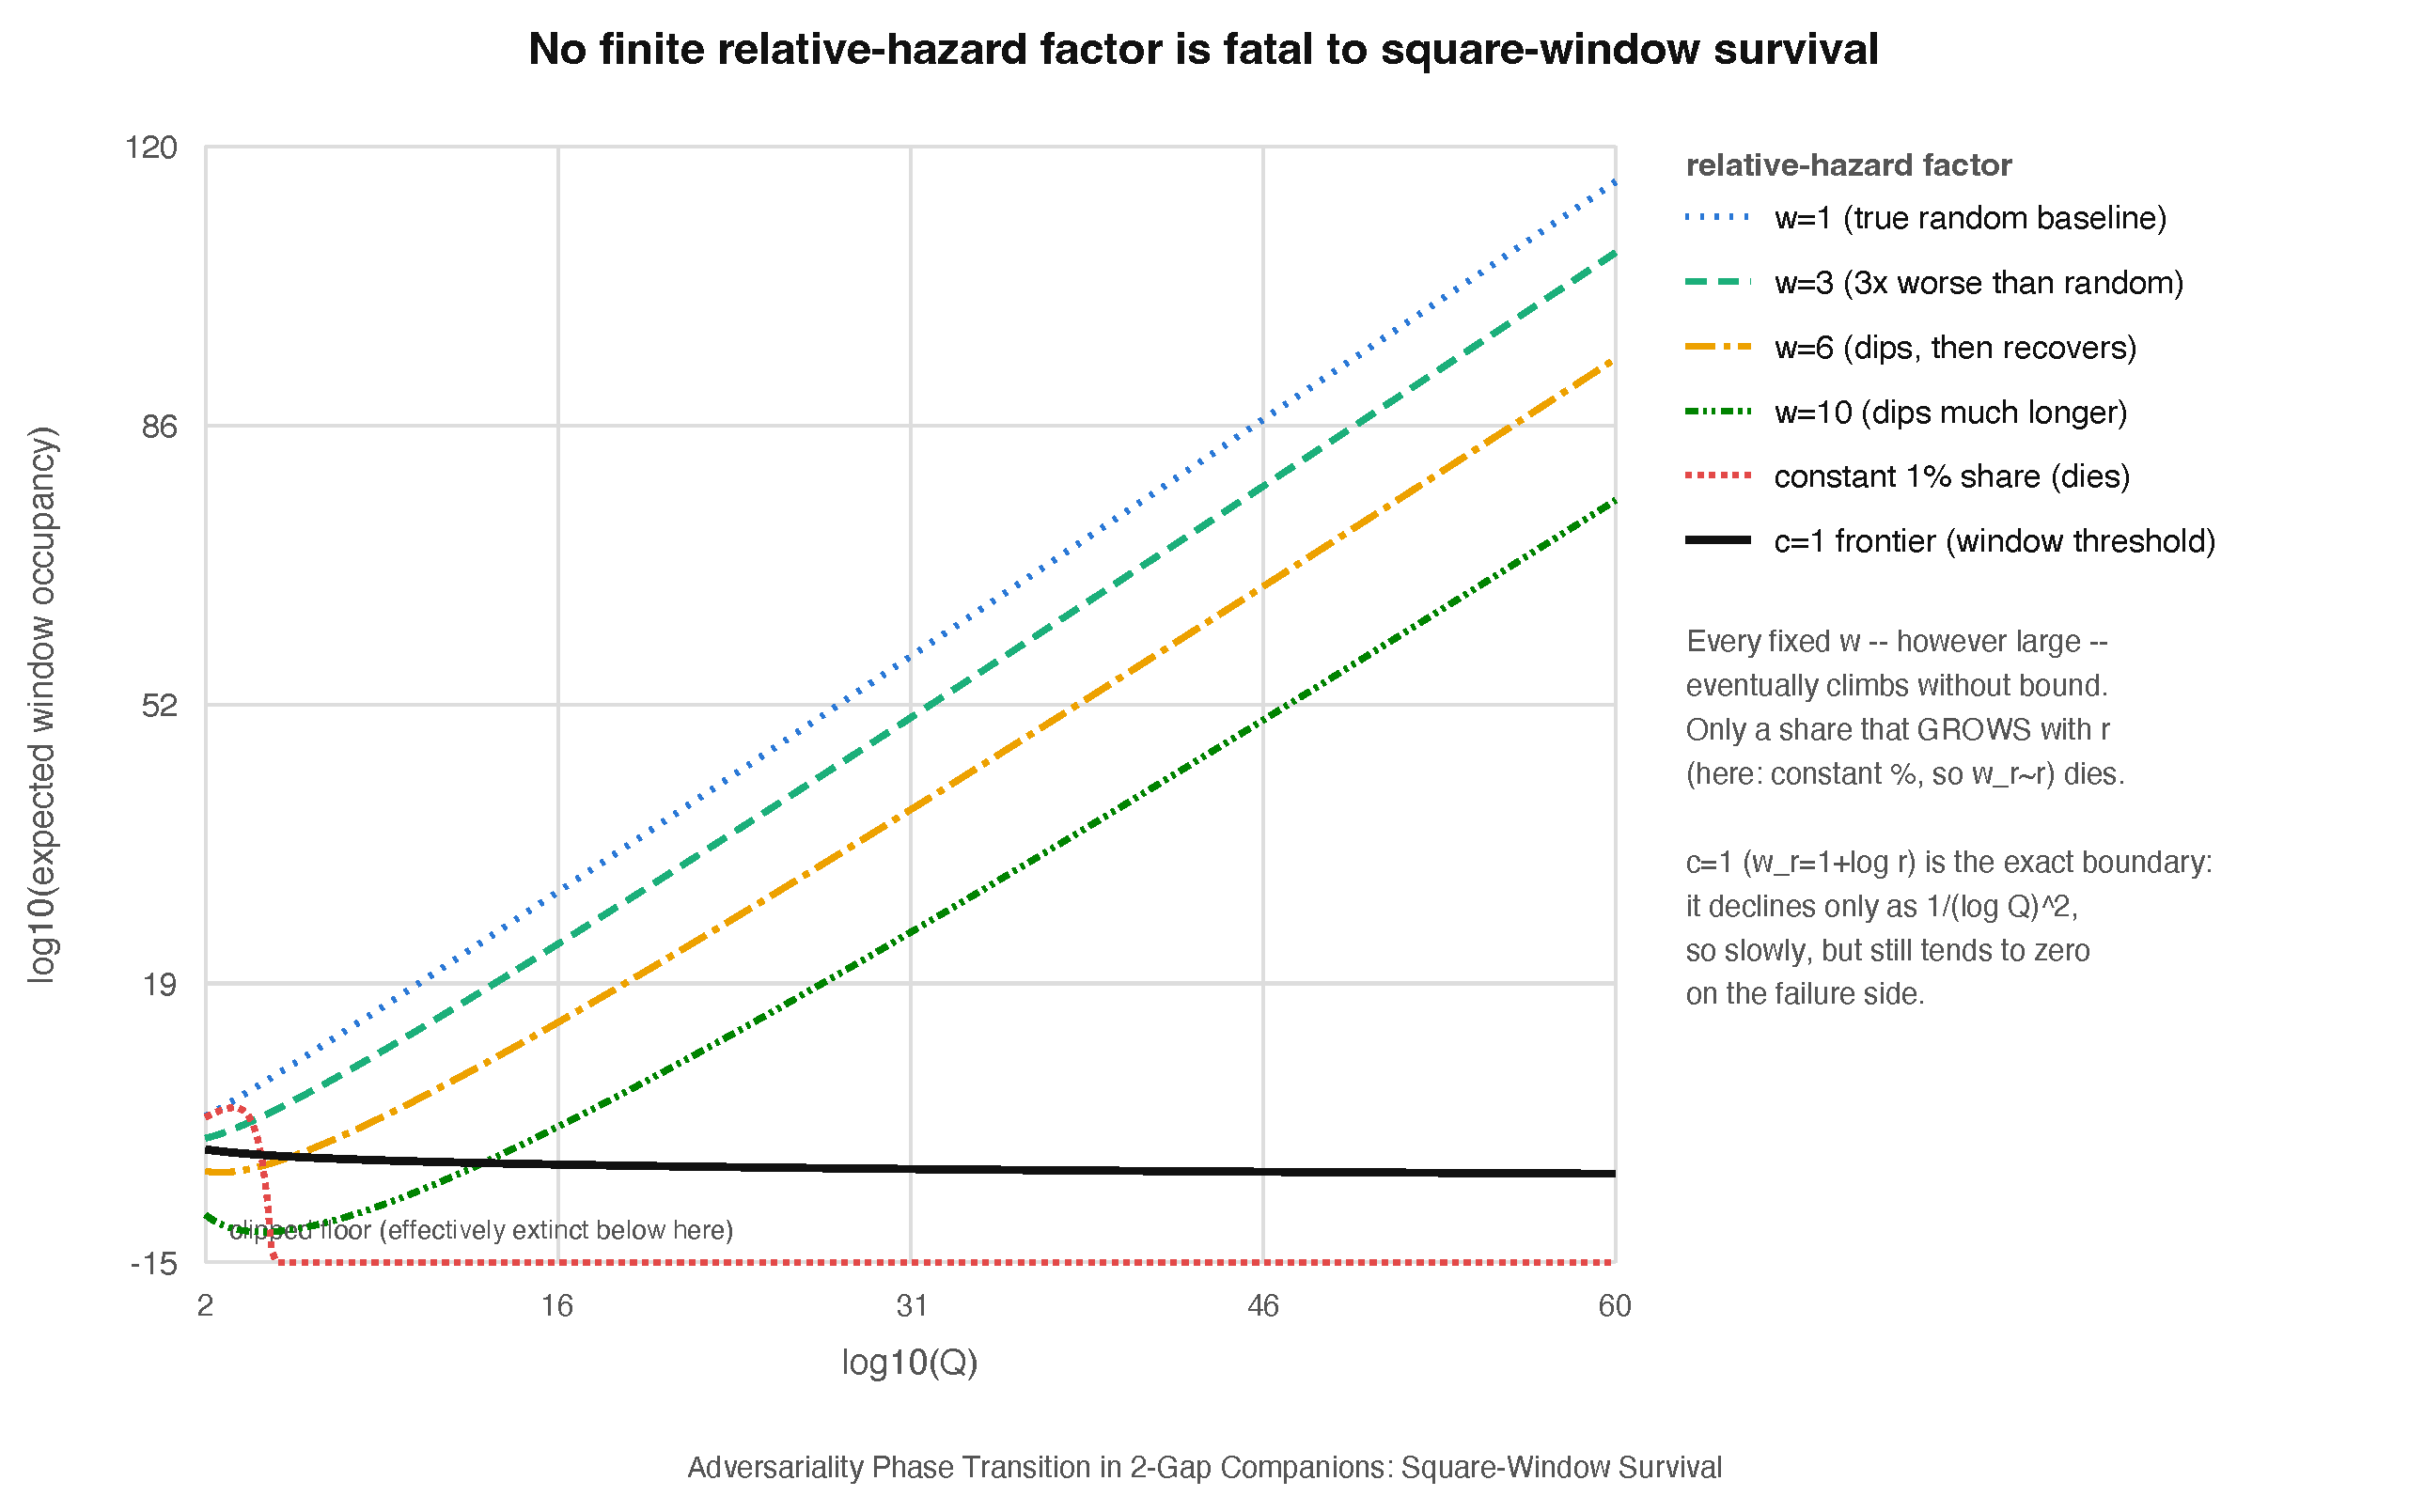
\includegraphics[width=\textwidth]{figures/phase-transition-window.pdf}
\caption{Square-window expected occupancy log10(lambda(Q)) on a log scale: every fixed relative-hazard factor w=1,3,6,10 eventually climbs without bound, a constant 1\% adversarial share collapses rapidly, and the exact c=1 boundary declines slowly to zero}
\end{figure}
\subsection{Logarithmically Growing Worsening Has Two Thresholds}
The first genuine transition appears when the worsening factor grows with the filter. Using the same supply, availability, and mixing premises as Section~3.4, we let the factor grow logarithmically and compare the reserve supplied by a square window with the much thinner reserve at one distinguished head.
\begin{equation*}
w_r=1+c\log r,
\qquad c\ge0.
\end{equation*}
The total local destruction rate is
\begin{equation*}
f_r
=\frac{2w_r}{r}
=\frac2r+2c\frac{\log r}{r}.
\end{equation*}
The random contribution supplies the first term, while the second is the growing excess. Prime summation gives
\begin{equation*}
\begin{aligned}
D_c(Q)
&=\sum_{r < Q}-\log(1-f_r)
&&[\text{Definition Of }D(Q)]\\
&=2\sum_{r < Q}\frac1r+2c\sum_{r < Q}\frac{\log r}{r}+O(1)
&&[\text{Substitution; Summable Remainder}]\\
&=2\log\log Q+2c\log Q+O(1).
&&[\text{Prime-Sum Asymptotics}]
\end{aligned}
\end{equation*}
Hence
\begin{equation*}
P_c(Q)
\asymp
\frac{C_c}{Q^{2c}(\log Q)^2}.
\qquad[\text{Exponentiation And Simplification}]
\end{equation*}
For a quadratic square-window supply,
\begin{equation*}
\lambda_c(Q)
\asymp
C_0\frac{Q^{2-2c}}{(\log Q)^2}.
\end{equation*}
Therefore
\begin{equation*}
\begin{aligned}
c < 1
&\Longrightarrow
\text{eventually nonempty square windows almost surely},\\
c\ge1
&\Longrightarrow
\text{square-window expectation tends to zero}.
\end{aligned}
\end{equation*}
For the head,
\begin{equation*}
\Pr(H_Q)
\asymp
\frac{C_c}{Q^{2c}(\log Q)^2}.
\end{equation*}
Summing over prime heads has the same convergence behavior as
\begin{equation*}
\int^\infty
\frac{dx}{x^{2c}(\log x)^3}.
\end{equation*}
Thus
\begin{equation*}
\begin{aligned}
c < \frac12
&\Longrightarrow
\text{infinitely many head events almost surely, with mixing},\\
c\ge\frac12
&\Longrightarrow
\text{only finitely many head events almost surely}.
\end{aligned}
\end{equation*}
The threshold is the Borel-Cantelli decision rule for the head, and the figure below evaluates it directly. It plots the cumulative sum of $\Pr(H_Q)$ over real enumerated primes up to $Q$, for $w_r=1+c\log r$ at $c=0.0,0.1,0.3,0.5,0.7,1.0$. Below the threshold the sum keeps climbing -- $c=0.0$ and $c=0.1$ clearly, $c=0.3$ more slowly but provably -- so there are infinitely many head events with mixing. At and above the threshold the sum flattens: $c=0.5$ only very slowly (it is the boundary itself), $c=0.7$ and $c=1.0$ quickly -- so there are only finitely many, almost surely.
\begin{figure}[htbp]
\centering
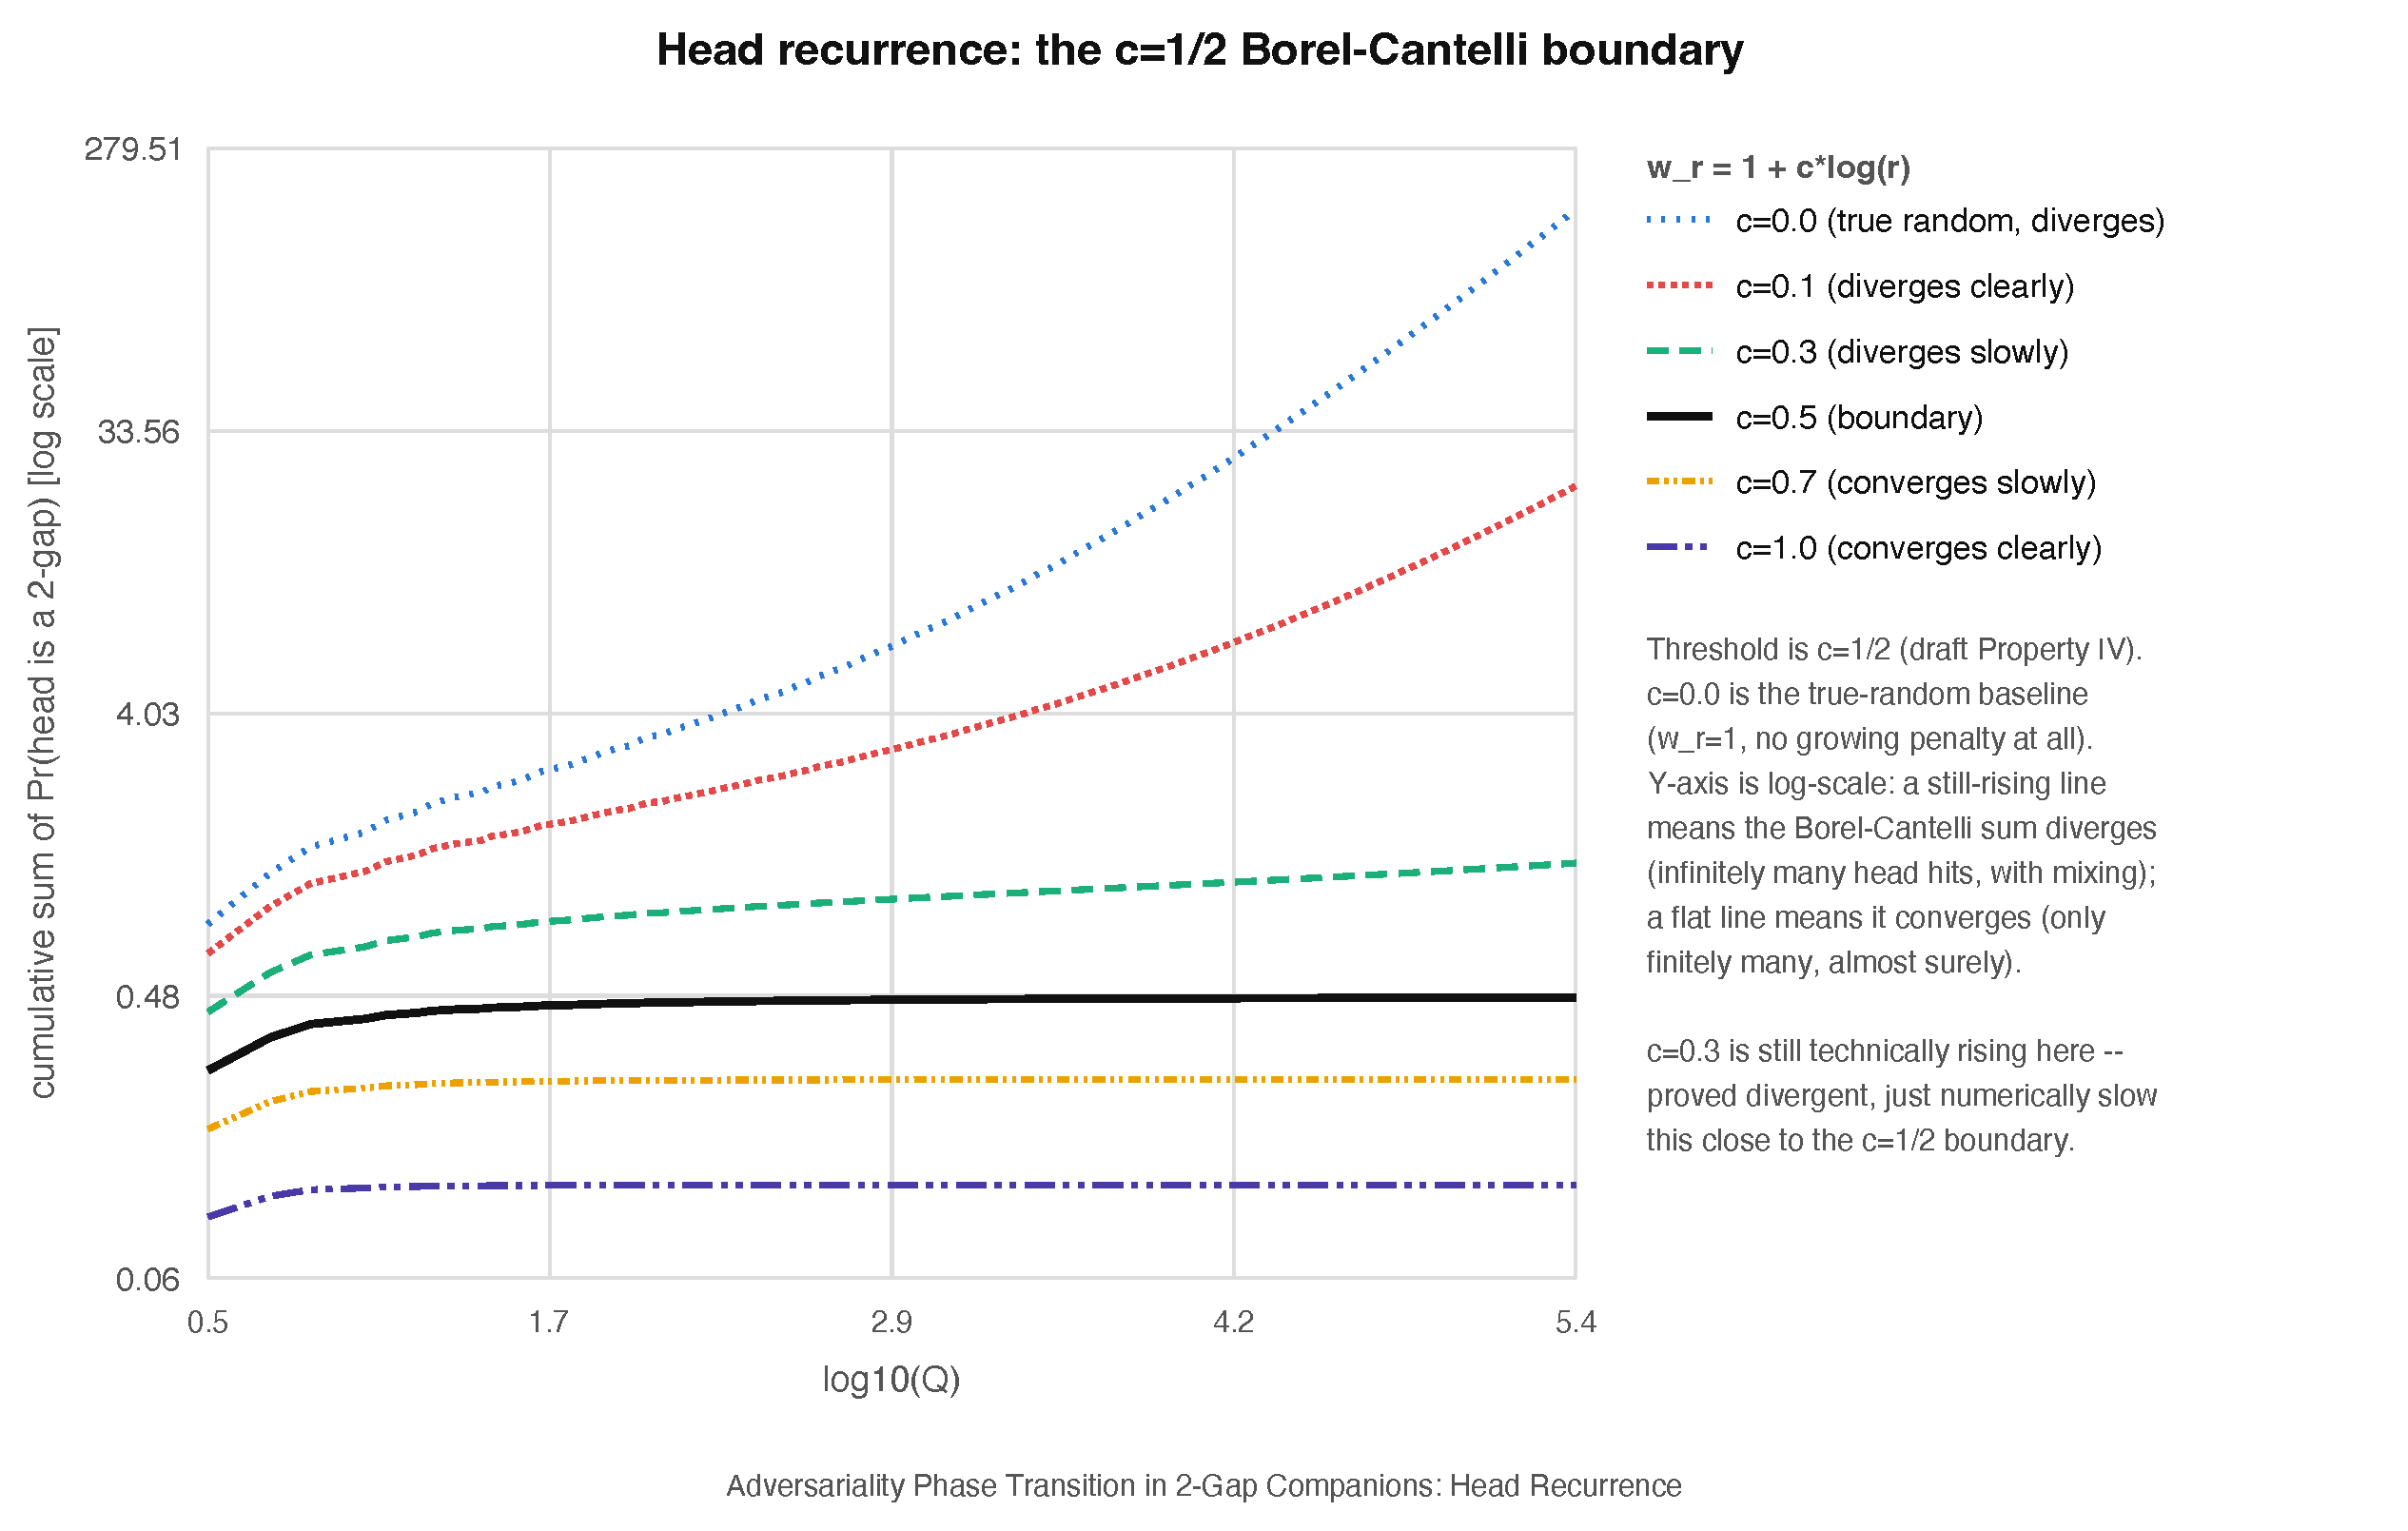
\includegraphics[width=\textwidth]{figures/phase-transition-head.pdf}
\caption{Cumulative sum of Pr(head is a 2-gap) over enumerated primes, log scale: c=0.0 and c=0.1 climb the whole way, c=0.3 climbs slowly, c=0.5 flattens only very slowly at the boundary, and c=0.7 and c=1.0 flatten quickly -- the c=1/2 Borel-Cantelli threshold}
\end{figure}
Equivalently, the robust relative-factor regimes are
\begin{equation*}
\begin{aligned}
w_r& < (1-\varepsilon)\log r
&&[\text{Square-Window Survival}],\\
w_r& < \left(\frac12-\varepsilon\right)\log r
&&[\text{Head Recurrence}],
\end{aligned}
\end{equation*}
up to the asymptotically negligible additive random baseline. In terms of the total segment destruction fraction,
\begin{equation*}
\begin{aligned}
f_r& < (2-\varepsilon)\frac{\log r}{r}
&&[\text{Square-Window Survival}],\\
f_r& < (1-\varepsilon)\frac{\log r}{r}
&&[\text{Head Recurrence}].
\end{aligned}
\qquad[\text{Q.E.D.}]
\end{equation*}
These are cumulative asymptotic regimes, not pointwise allowances that reset at each filter. Irregular schedules must be evaluated through $D(Q)$.
The complete proof record appears in Appendix~A.4.
\subsection{Relative-to-Random Phase Diagram}
The answer is not a maximum fixed percentage. It is a growth-rate boundary for the realized local damage relative to the random benchmark.
\begin{longtable}{@{}>{\raggedright\arraybackslash}p{0.26\textwidth}>{\raggedright\arraybackslash}p{0.15\textwidth}>{\raggedright\arraybackslash}p{0.25\textwidth}>{\raggedright\arraybackslash}p{0.24\textwidth}@{}}
\toprule
Realized relative factor & Total local destruction & Square windows & Head 2-gaps \\
\midrule
$w_r=1$ & $2/r$ & Eventually nonempty almost surely & Infinitely often with mixing \\
Any fixed finite $w_r=w$ & $2w/r$ & Eventually nonempty almost surely & Infinitely often with mixing \\
$w_r=1+c\log r$, $0\le c < 1/2$ & $2/r+2c\log r/r$ & Eventually nonempty almost surely & Infinitely often with mixing \\
$w_r=1+c\log r$, $1/2\le c < 1$ & $2/r+2c\log r/r$ & Eventually nonempty almost surely & Only finitely often almost surely \\
$w_r=1+c\log r$, $c\ge1$ & $2/r+2c\log r/r$ & Expected population tends to zero & Only finitely often almost surely \\
$f_r=1$ at a tracked step & $1$ & That tracked cohort is lost & That candidate is lost \\
\bottomrule
\end{longtable}
Consequently, there is \textbf{no largest finite constant multiple of random}. For square-window survival, the filter may become almost $\log r$ times worse than random; for infinitely recurring head 2-gaps, it may become almost $\tfrac12\log r$ times worse. In total local-destruction terms, the robust sufficient regimes are respectively
\begin{equation*}
f_r < (2-\varepsilon)\frac{\log r}{r}
\qquad\text{and}\qquad
f_r < (1-\varepsilon)\frac{\log r}{r}.
\end{equation*}
These conclusions concern damage realized inside the tracked segment. A small global adversarial budget can still cause $f_r=1$ if it is allocated with enough target information; the allocation theorem in Section~5 isolates that second axis.
